\documentclass[letterpaper]{article}
\usepackage{amssymb}
\usepackage{fullpage}
\usepackage{changepage}
\usepackage{amsmath}
\usepackage{epsfig,float,alltt}
\usepackage{psfrag,xr}
\usepackage[T1]{fontenc}
\usepackage{url}
\usepackage{pdfpages}
\usepackage{epstopdf}
\usepackage[framed,numbered,autolinebreaks,useliterate]{mcode}
\usepackage{indentfirst}
\usepackage{tikz,mathpazo}
%\includepdfset{pagecommand=\thispagestyle{fancy}}
\author{Fan Bu\\ UMID: 68836435\\ Unique Name: fanbu}
\title{EECS 442 Computer Vision, Midterm Exam}

\begin{document}
\date{11/02/2016}
\maketitle

\newcommand{\trace}{\mathrm{trace}}
\newcommand{\real}{\mathbb R}  % real numbers  {I\!\!R}
\newcommand{\nat}{\mathbb N}   % Natural numbers {I\!\!N}
\newcommand{\cp}{\mathbb C}    % complex numbers  {I\!\!\!\!C}
\newcommand{\ds}{\displaystyle}
\newcommand{\mf}[2]{\frac{\ds #1}{\ds #2}}
\newcommand{\spanof}[1]{\textrm{span} \{ #1 \}}
\newcommand{\sol}[0]{\textbf{Solution: }}
\newcommand{\pf}[0]{\textbf{Proof:}}
\newcommand{\rme}[0]{\textrm{e}}
\newcommand{\Null}[1]{\textrm{Null}\{#1\}}
\parindent 0pt
%%%%%%%%%%%%%%%%%%%%%%%%%%%%%%%%%%%%%%%%%%%%%%%%%%%%%%%%%%%%%%%%%%%%%%%%%%%%%%%
% Solution for Question 1 begins here - by Fan Bu
%%%%%%%%%%%%%%%%%%%%%%%%%%%%%%%%%%%%%%%%%%%%%%%%%%%%%%%%%%%%%%%%%%%%%%%%%%%%%%%
\section*{Question 1, Transformations}
\subsection*{(a)}
Show that these rotations produce different values of p'\\
Case 1, first rotate $\beta$ around y axis, then rotate $\gamma$ around z axis.
\begin{align*}
p_1'&=R_z(\gamma)R_y(\beta)p\\
&=\begin{bmatrix}
cos(\gamma)& -sin(\gamma)& 0\\
sin(\gamma)&  cos(\gamma)& 0\\
0&           0& 1
\end{bmatrix}
\begin{bmatrix}
cos(\beta) & 0 & sin(\beta)\\
0 & 1 & 0\\
-sin(\beta)& 0& cos(\beta)
\end{bmatrix}p\\
&=\begin{bmatrix}
cos(\beta)cos(\gamma)& -sin(\gamma)& cos(\gamma)sin(\beta)\\
cos(\beta)sin(\gamma)&  cos(\gamma)& sin(\beta)sin(\gamma)\\
-sin(\beta)&           0& cos(\beta)
\end{bmatrix}p
\end{align*}
Case 2, first rotate $\gamma$ around z axis, then rotate $\beta$ around y axis.
\begin{align*}
p_2'&=R_y(\beta)R_z(\gamma)p\\
&=\begin{bmatrix}
cos(\beta) & 0 & sin(\beta)\\
0 & 1 & 0\\
-sin(\beta)& 0& cos(\beta)
\end{bmatrix}
\begin{bmatrix}
cos(\gamma)& -sin(\gamma)& 0\\
sin(\gamma)&  cos(\gamma)& 0\\
0&           0& 1
\end{bmatrix}p\\
&=\begin{bmatrix}
cos(\beta)cos(\gamma)& -cos(\beta)sin(\gamma)& sin(\beta)\\
sin(\gamma)&            cos(\gamma)&         0\\
-cos(\gamma)sin(\beta)&  sin(\beta)sin(\gamma)& cos(\beta)\\
\end{bmatrix}p
\end{align*}
Compare case 1 and case 2, we can easily conduct that the two result $p_1'$ and $p_2'$ are different.\\
\subsection*{(b)}
If $\beta=0$,
\begin{align*}
R_x(\alpha)R_y(\beta)R_z(\gamma)&=R_x(\alpha)R_y(0)R_z(\gamma)\\
&=\begin{bmatrix}
1 & 0 & 0\\
0 & cos(\alpha) & -sin(\alpha)\\
0 & sin(\alpha) & cos(\alpha)
\end{bmatrix}
\begin{bmatrix}
1 & 0 & 0\\
0 & 1 & 0\\
0 & 0 & 1
\end{bmatrix}
\begin{bmatrix}
1 & 0 & 0\\
0 & cos(\gamma) & -sin(\gamma)\\
0 & sin(\gamma) & cos(\gamma)
\end{bmatrix}\\
&=\begin{bmatrix}
1 & 0 & 0\\
0 & cos(\alpha)cos(\gamma)-sin(\alpha)sin(\gamma) & -cos(\alpha)sin(\gamma)-sin(\alpha)cos(\gamma)\\
0 & sin(\alpha)cos(\gamma)+cos(\alpha)sin(\gamma) & -sin(\alpha)sin(\gamma)+cos(\alpha)cos(\gamma)
\end{bmatrix}\\
(due\ to\ some\ trigonometric\ identities)&=\begin{bmatrix}
1 & 0 & 0\\
0 & cos(\alpha+\gamma) & -sin(\alpha+\gamma)\\
0 & sin(\alpha+\gamma) & cos(\alpha+\gamma)
\end{bmatrix}
\end{align*}
Since the result only determines on $(\alpha+\gamma)$, only one degree of freedom is left.\\
\clearpage

\section*{Question 2, Panoramic Imaging Theory}
\subsection*{(a)}
Prove that the homographic transformation $H$ defined by $p_1',p_2',p_3',p_4'$ and $p_1,p_2,p_3,p_4$ can be expressed as $H=KRK^{-1}$\\
Let $P$ be the world coordinate, then\\
$$p=K\begin{bmatrix}
I & 0\\
\end{bmatrix}P$$
$$p'=K\begin{bmatrix}
R & 0\\
\end{bmatrix}P$$
We may express $p'$ as the following:\\
\begin{align*}
p'&=KR\begin{bmatrix}
I & 0\\
\end{bmatrix}P\\
&=KRI\begin{bmatrix}
I & 0\\
\end{bmatrix}P\\
&=KR(K^{-1}K)\begin{bmatrix}
I & 0\\
\end{bmatrix}P\\
&=KRK^{-1}(K\begin{bmatrix}
I & 0\\
\end{bmatrix}P)\\
(since\ p=K\begin{bmatrix}
I & 0\\
\end{bmatrix}P)&= (KRK^{-1})p\\
&=Hp
\end{align*}
Thus, $H$ can be expressed as $H=KRK^{-1}$.\\
\clearpage
\section*{Question 3, Computing H}
Briefly deduce the DTL algorithm.\\
Since we are working in homogeneous coordinates, the relationship between two corresponding points $x$ and $x'$ can be re-written as:\\
\begin{equation}
c\begin{bmatrix}
u\\
v\\
1
\end{bmatrix}
=H\begin{bmatrix}
x\\
y\\
1
\end{bmatrix}
\label{equaion1}
\end{equation}

where $c$ is any non-zero constant, $[u,v,1]^T$ represents $x'$, $[x,y,1]^T$ represents $x$, and $H=\begin{bmatrix}
h_1 & h_2& h_3\\
h_4 & h_5& h_6\\
h_7 & h_8& h_9
\end{bmatrix}$\\
Dividing the first row of equation \ref{equaion1} by the third row and the second row by the third row we get the following two equations:\\
\begin{equation}
-h_1x-h_2y-h_3+(h_7x+h_8y+h_9)u=0
\label{equaion2}
\end{equation}
\begin{equation}
-h_4x-h_5y-h_6+(h_7x+h_8y+h_9)u=0
\label{equaion3}
\end{equation}\\
Equations \ref{equaion2} and \ref{equaion3} can be written in matrix form as:\\
$$A_ih=0$$
where $A_i=\begin{bmatrix}
-x & -y & -1 & 0 & 0 & 0 & ux& uy& u\\
0 & 0 & 0 & -x & -y & -1 & vx& vy& v
\end{bmatrix}$ and $h=\begin{bmatrix}
h_1 & h_2& h_3 & h_4 & h_5& h_6 & h_7 & h_8& h_9
\end{bmatrix}^T$.\\

Since each point correspondence provides 2 equations, 4 correspondences are sufficient to solve for the 8 degrees of freedom of $H$. The restriction is
that no 3 points can be collinear (i.e., they must all be in "general position").
For $2\times 9 \ A_i$ matrices(one per point correspondence) can be stacked on top
of one another to get a single $8\times 9$ matrix $A$.\\

In some cases, we may use more than 4 correspondences to ensure a more robust solution, then we may use SVD to solve for the filnal $H$, as commented in my codes.\\

Since we only have 4 points here, the 1D null space of $A$ is the solution space for
$h$(i.e. $h=null(A)$). \\

The final result of $H$ is shown below, where $H$ projects points as $X_2=HX_1$:\\
$$
H=\begin{bmatrix}
   -1.8619  & -0.5207 & 591.3803\\
   -0.8226  & -2.2354 & 441.5196\\
   -0.0044  & -0.0046 &   1.0000
   \end{bmatrix}
   $$
\\
And codes are attached as following:
\begin{lstlisting}
function main()
clear all;
close all;
clc;
[points1 points2] = readPoints('4points.txt')
H=DLT_H(points1,points2)
end
function H=DLT_H(x1,x2)
[n1, ~]=size(x1);
[n2, ~]=size(x2);
if n1~=n2
    error=char('x1 and x2 does not match!')
   return
else
    n=n1;
end

%Build the matrix A such that,
% A_i=[-x,-y,-1,0,0,0,ux,uy,u;
%     0,0,0,-x,-y,-1,vx,vy,v]
A=zeros(2*n,9);
for i = 1:n
    A(2*i-1,1:3)=[-x1(i,1),-x1(i,2),-1];
    A(2*i-1,7:9)=[x2(i,1)*x1(i,1),x2(i,1)*x1(i,2),x2(i,1)];
    A(2*i,4:6)=[-x1(i,1),-x1(i,2),-1];
    A(2*i,7:9)=[x2(i,2)*x1(i,1),x2(i,2)*x1(i,2),x2(i,2)];
end
h=null(A);
H=zeros(3,3);
H(1,:)=h(1:3);
H(2,:)=h(4:6);
H(3,:)=h(7:9);
H=H/H(3,3);

% % If more than 4 points, we can use SVD to solve H
% [u,s,v] = svd(A,0);
% vv=v(:,9);
% for i=1:3
% H(1,i)=vv(i);
% end
% for i=1:3
% H(2,i)=vv(i+3);
% end
% for i=1:3
% H(3,i)=vv(i+6);
% end
%
% % let rank(F)=2
% [u,s,v] = svd(H);
% H = H - u(:,3)*s(3,3)*transpose(v(:,3));
% H = H/H(3,3);
end
\end{lstlisting}
\clearpage

\section*{Question 4, Convolution}
The Original Picture is shown below in Fig \ref{original_image}:\\
\begin{figure}[H]
\begin{center}
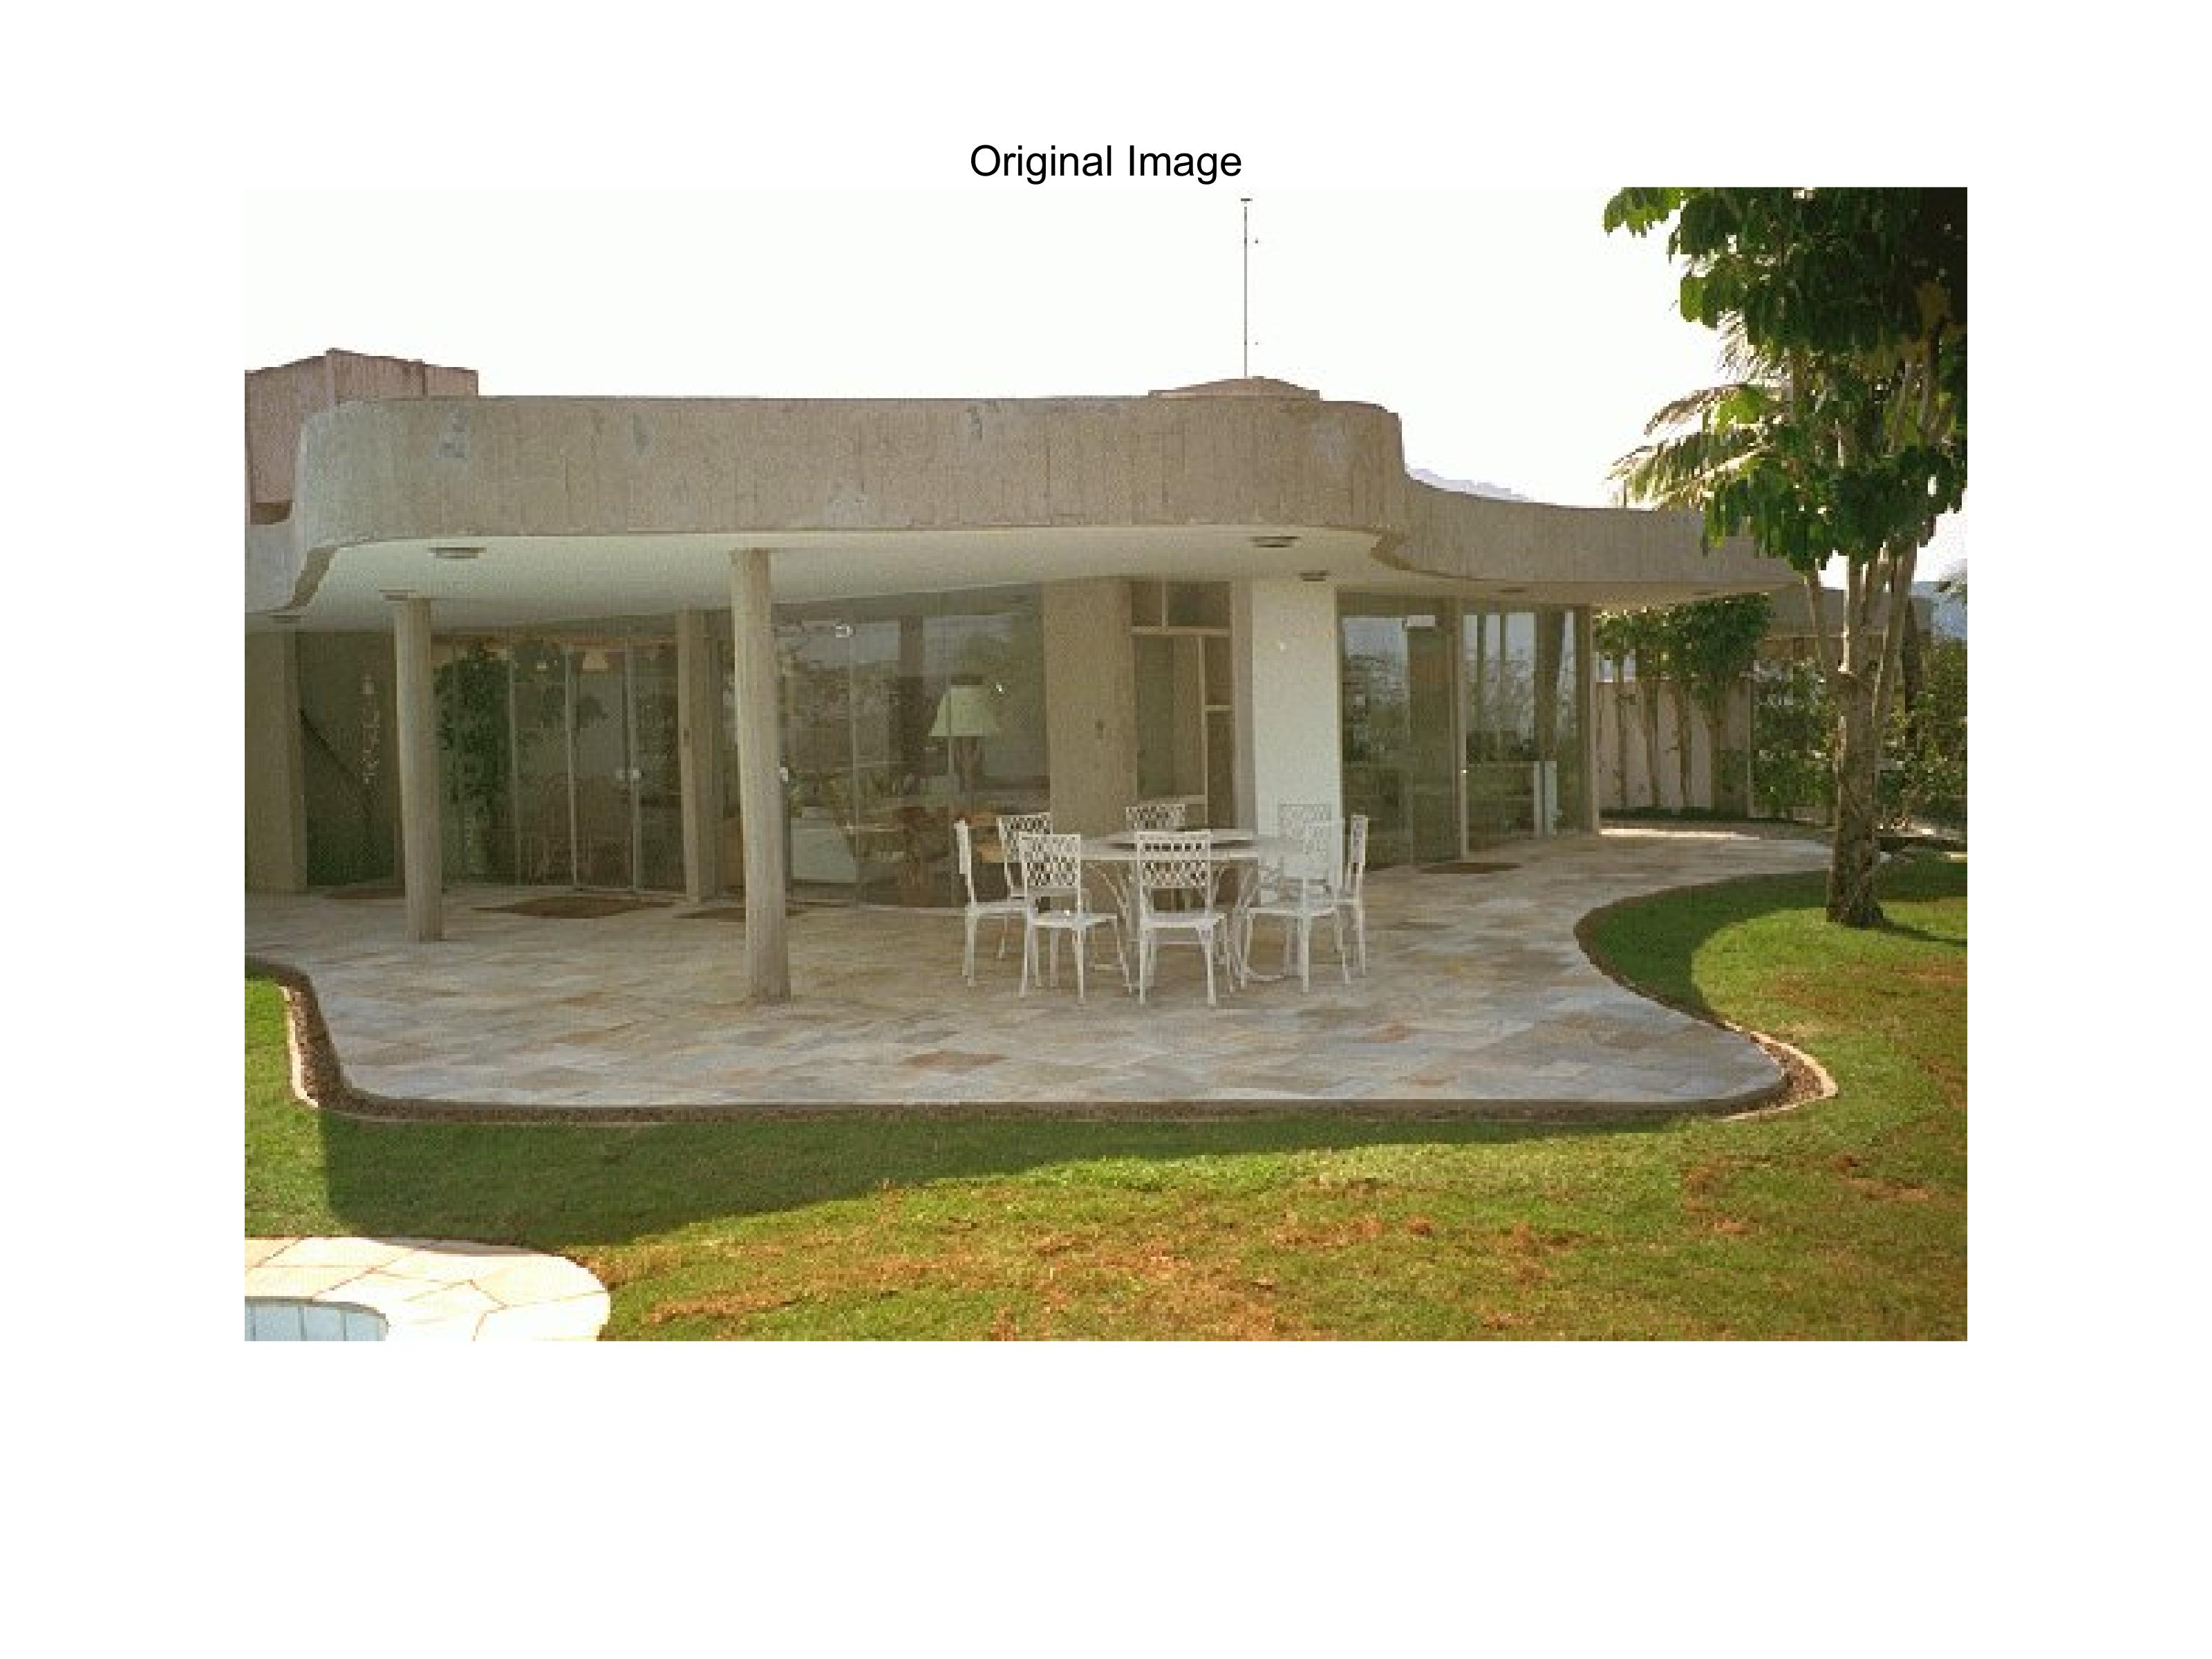
\includegraphics[width = 16cm]{original_image.jpeg}
\caption{Original Image}
\label{original_image}
\end{center}
\end{figure}

In Gaussian Blurring, the window size depends on the value of $\sigma$. Usually, we set the filter half-width to about $3\sigma$, so I set the window size to about "$6\sigma+1$" in my codes.\\
\subsection*{Visual results}
The blurred result of three different $\sigma$ values are shown below, with $\sigma=1$, $\sigma=3$, $\sigma=5$ in Fig \ref{Question4_sigma_1},Fig \ref{Question4_sigma_3}, Fig \ref{Question4_sigma_5} respectively.\\
\begin{figure}[H]
\begin{center}
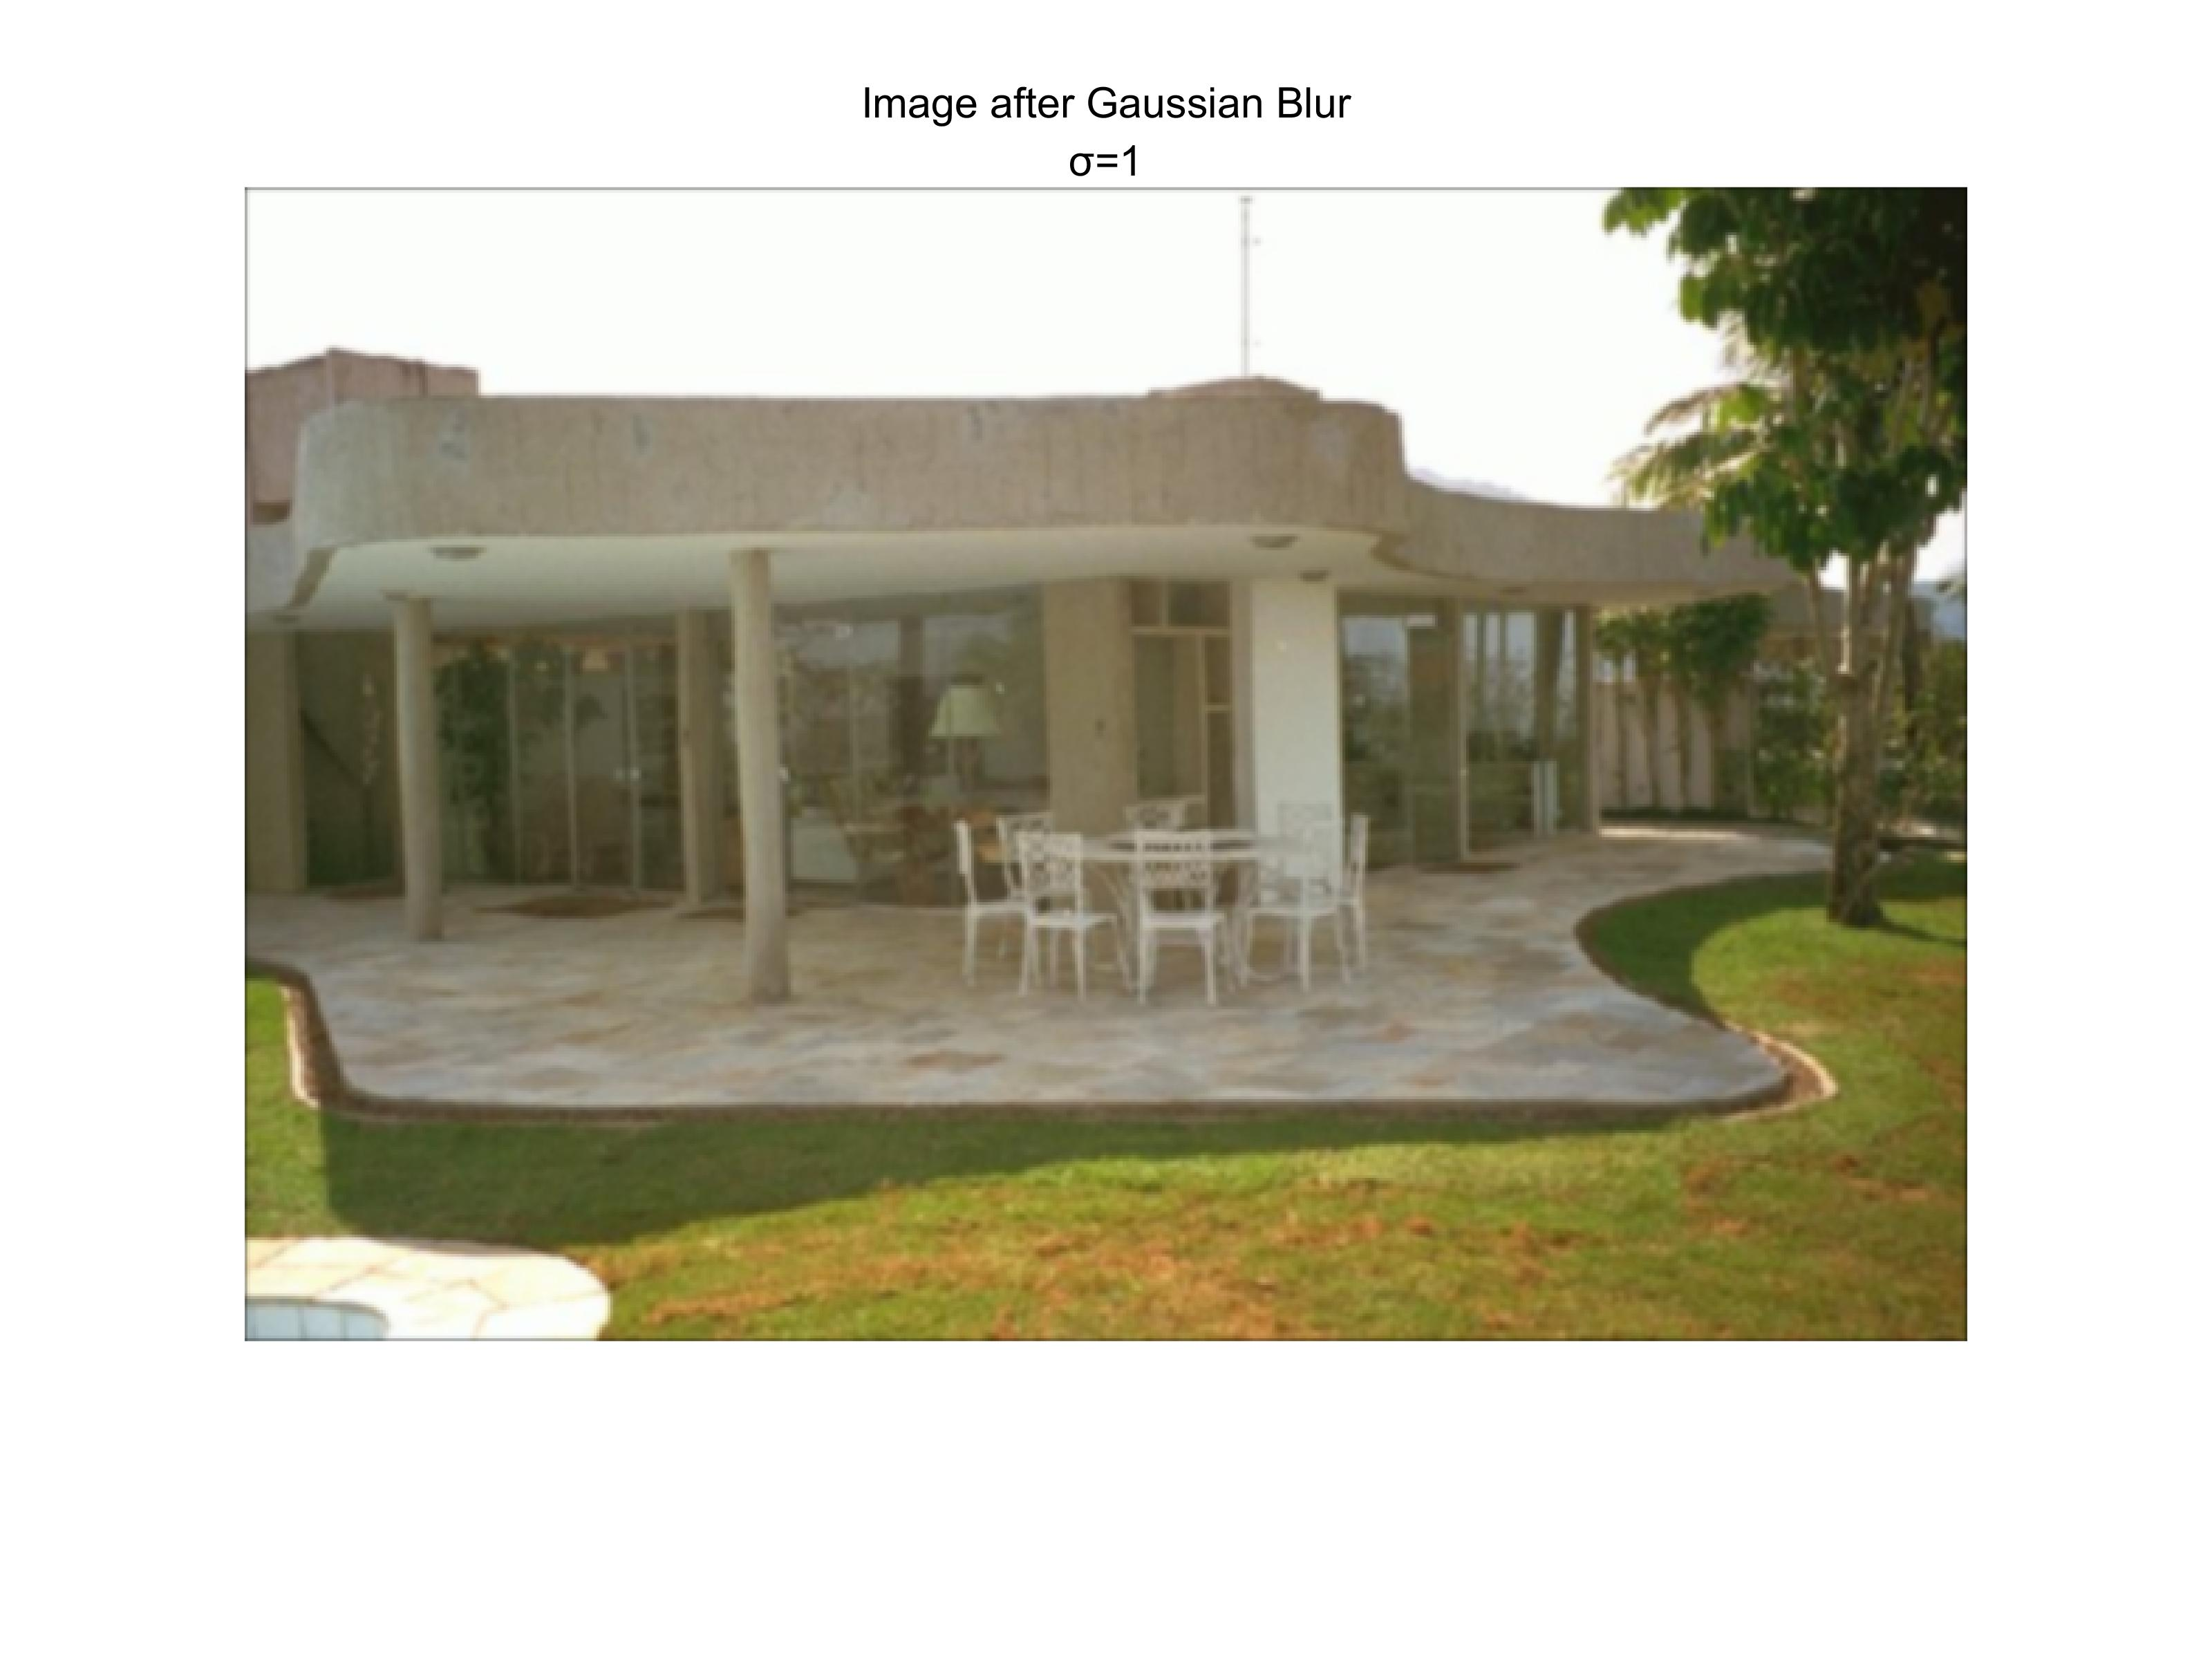
\includegraphics[width = 12cm]{Question4_sigma_1.jpeg}
\caption{Gaussian Blur, $\sigma=1$}
\label{Question4_sigma_1}
\end{center}
\end{figure}
\begin{figure}[H]
\begin{center}
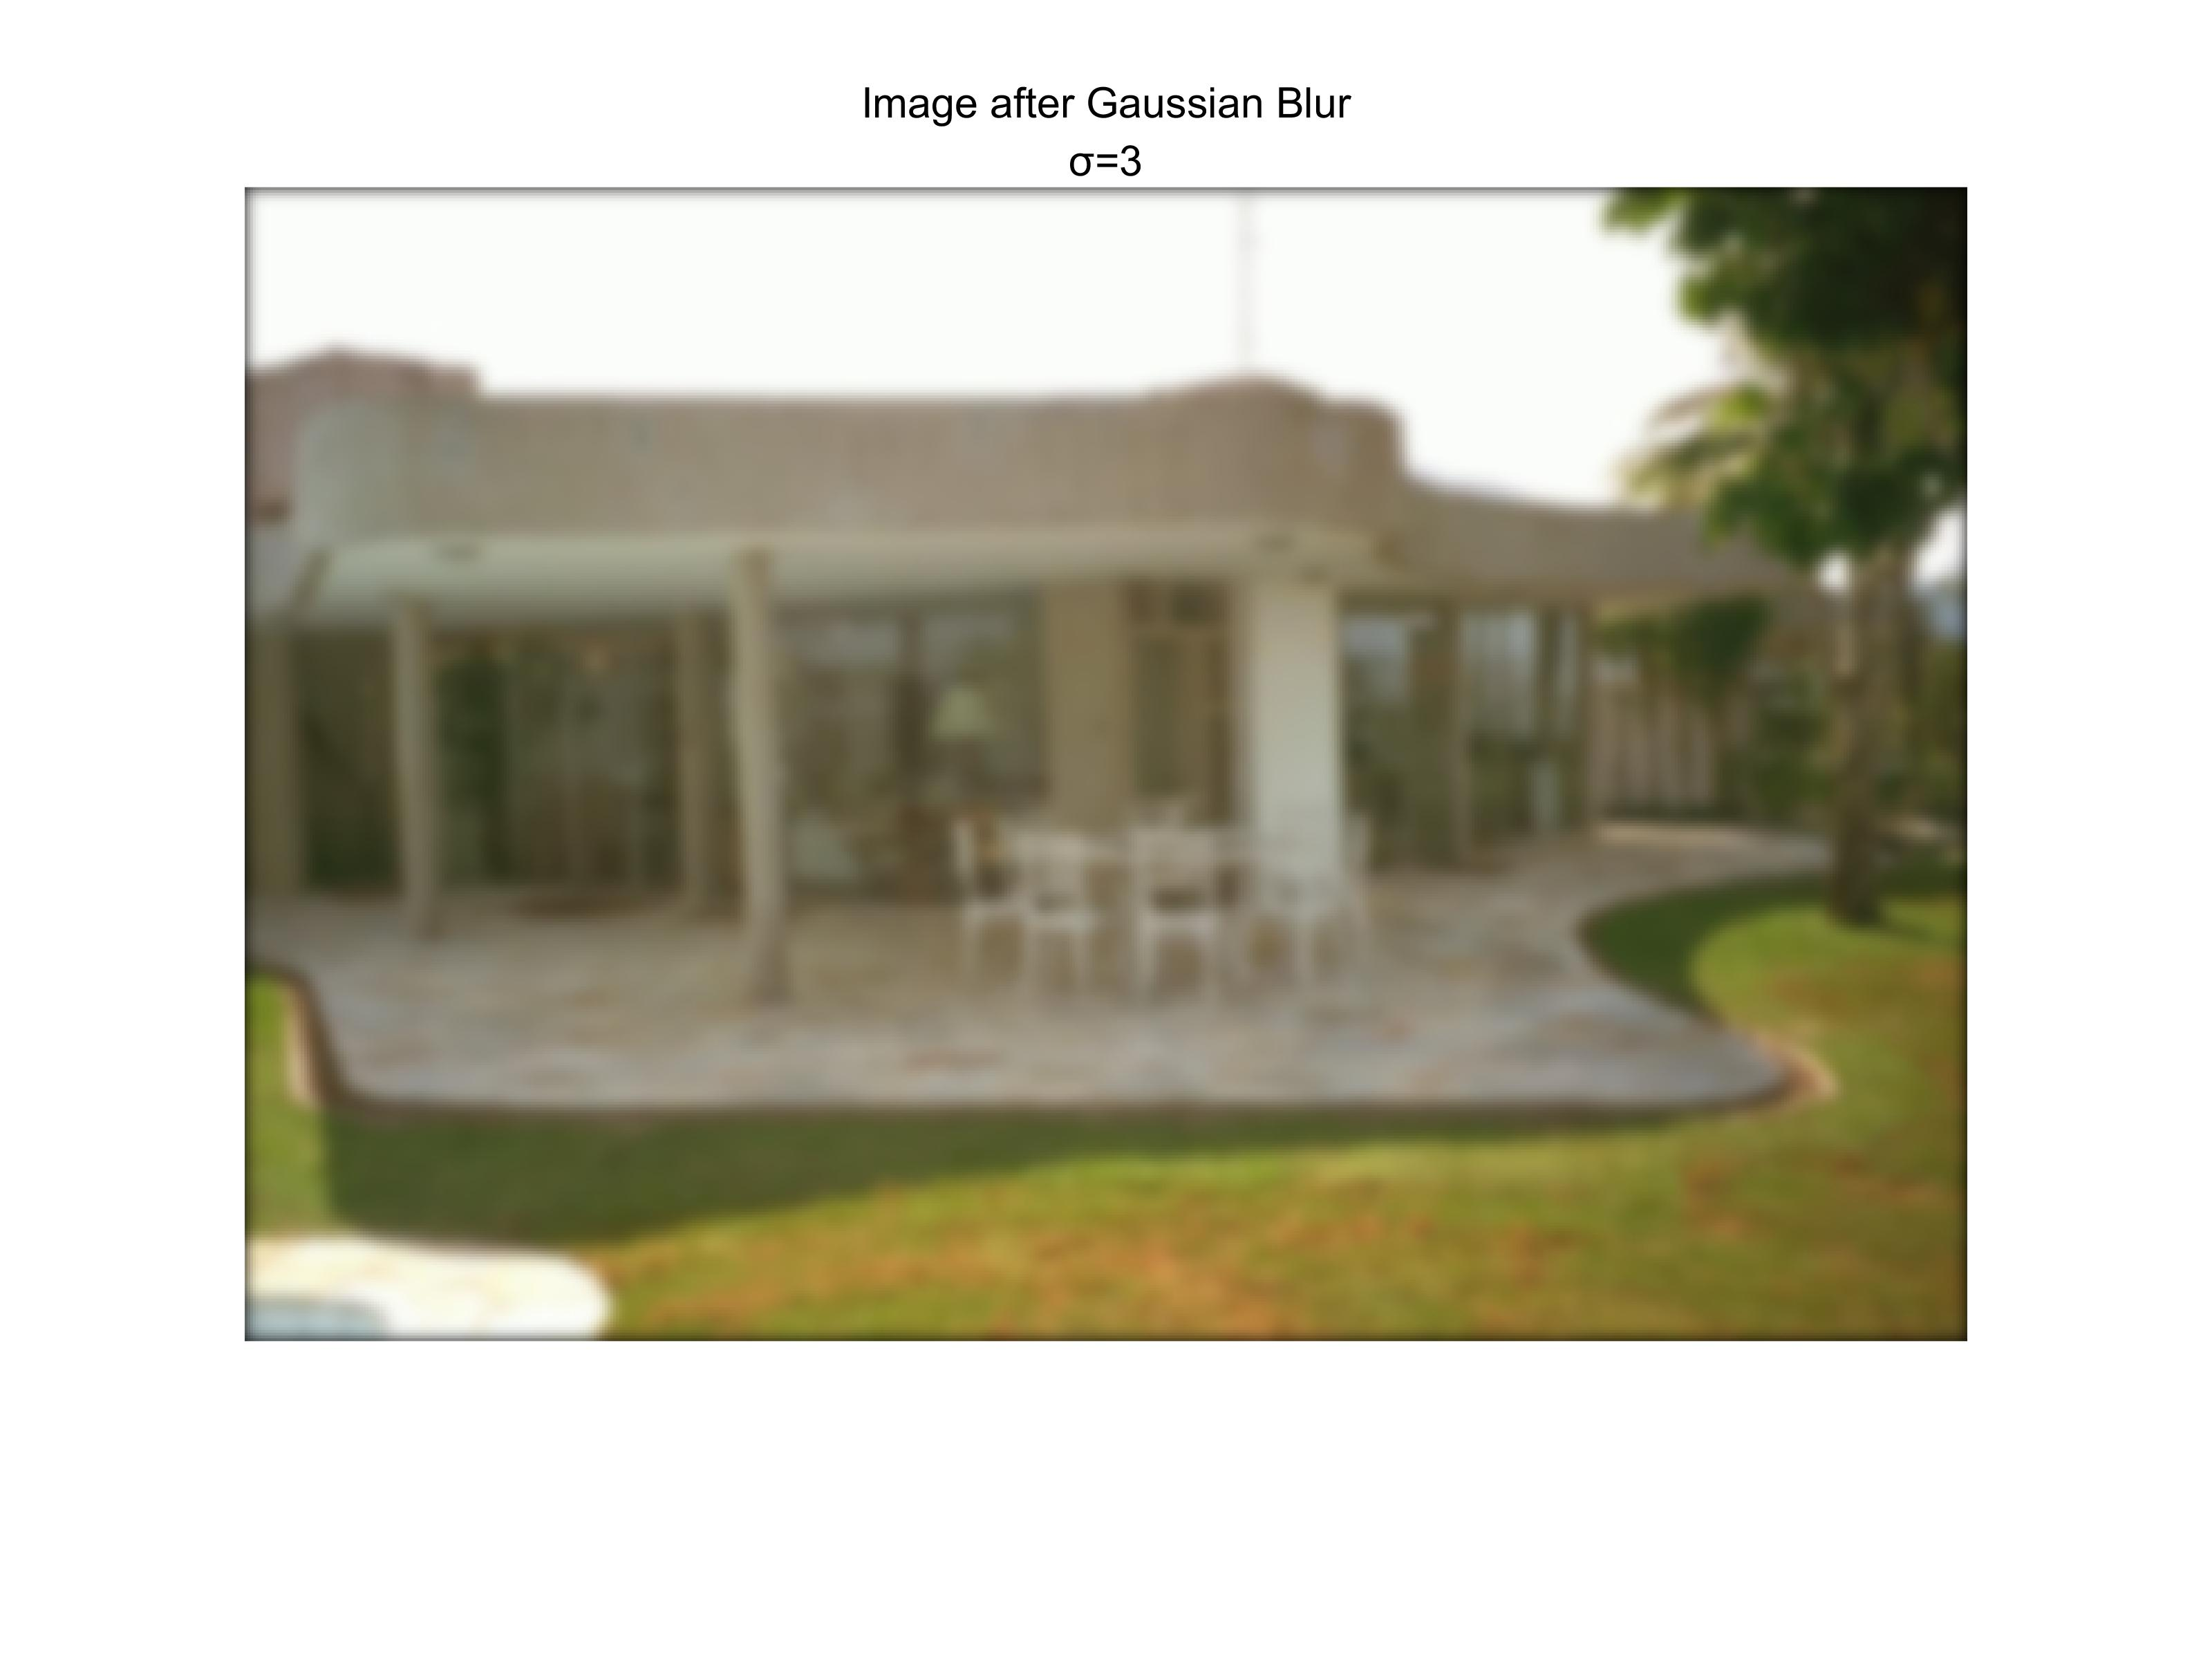
\includegraphics[width = 12cm]{Question4_sigma_3.jpeg}
\caption{Gaussian Blur, $\sigma=3$}
\label{Question4_sigma_3}
\end{center}
\end{figure}
\begin{figure}[H]
\begin{center}
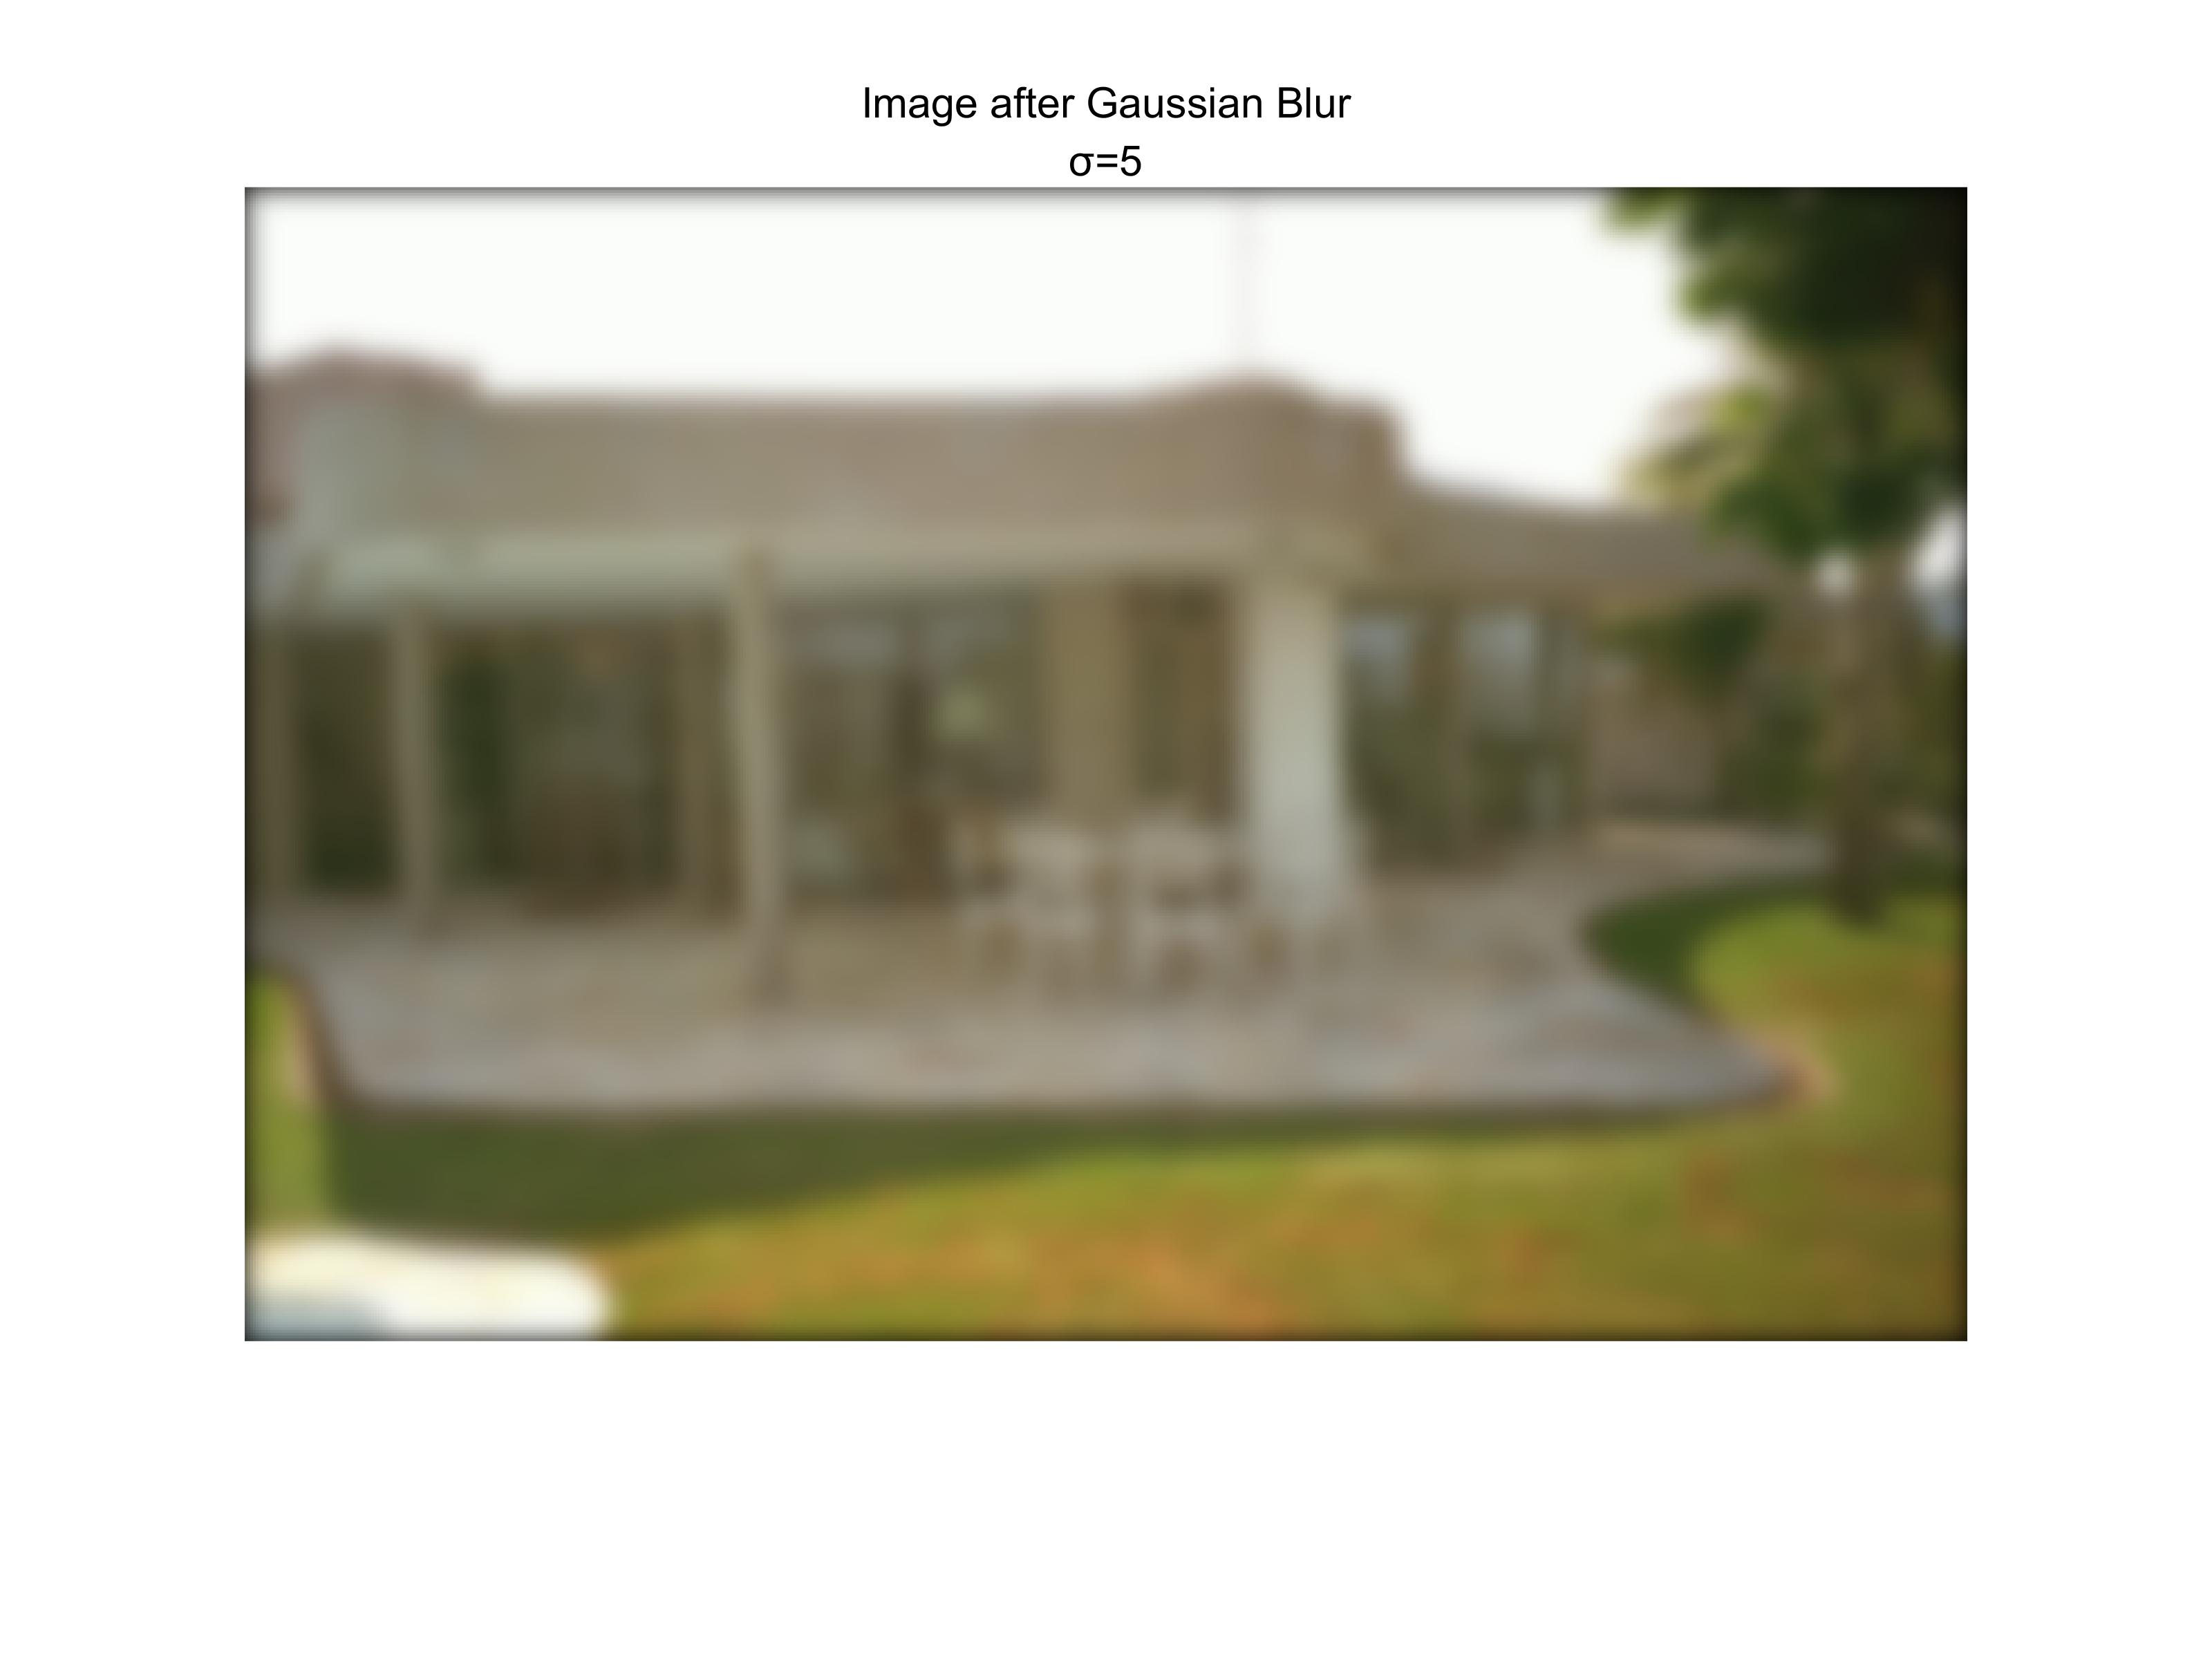
\includegraphics[width = 12cm]{Question4_sigma_5.jpeg}
\caption{Gaussian Blur, $\sigma=5$}
\label{Question4_sigma_5}
\end{center}
\end{figure}
\subsection*{Comments about my results}
Note from the result that, as we increase the value of $\sigma$, the image becomes more blur or more smoothed. Because when $\sigma$ gets larger, the curve of the normal distribution becomes more flat, so that the neighbourhoods of a pixel are valued more in the new image. \\

Meanwhile, we also find that the black edge of a picture extends as $\sigma$ increases. This is because of the way I extend the original picture while applying my Gaussian kernel. To calculate new pixels on the edge, I extends the original picture by half-width of the kernel window and set the extended pixels value equals 0, which means I set the extended pixels color to black. Therefore, the larger the $\sigma$, the more black pixels on the edge were calculated, hence the wider the black edge is shown in the new image.\\
\subsection*{Source code}
Codes are attached below:\\
\begin{lstlisting}
function main
clear all;
close all;
clc;
image_name='garden1.jpg';
% Show Original Image
figure;
hold on;
imshow(image_name);
title({['Original Image']});
axis equal;
print(gcf,'-djpeg' ,strcat('original_image.jpeg'),'-r400')
% Choose Standard Deviation (sigma value = 1)
sigma = 1;
blur_image=Gau_blur(sigma,image_name);
figure;
title({['Image after Gaussian Blur'];
    ['��=',num2str(sigma)]});
hold on;
imshow(blur_image);
axis equal;
print(gcf,'-djpeg' ,strcat('Question4_sigma_',num2str(sigma),'.jpeg'),'-r400')

% Choose Standard Deviation (sigma value = 3)
sigma = 3;
blur_image=Gau_blur(sigma,image_name);
figure;
title({['Image after Gaussian Blur'];
    ['��=',num2str(sigma)]});
hold on;
imshow(blur_image);
axis equal;
print(gcf,'-djpeg' ,strcat('Question4_sigma_',num2str(sigma),'.jpeg'),'-r400')

% Choose Standard Deviation (sigma value = 5)
sigma = 5;
blur_image=Gau_blur(sigma,image_name);
figure;
title({['Image after Gaussian Blur'];
    ['��=',num2str(sigma)]});
hold on;
imshow(blur_image);
axis equal;
print(gcf,'-djpeg' ,strcat('Question4_sigma_',num2str(sigma),'.jpeg'),'-r400')
end

function blur_image=Gau_blur(sigma,image_name)
% Read in the Image
Image = imread(image_name);
% Change Format to Double
Img = double(Image);
% Calculate the half value of Kernel size
half_size=floor(3*sigma);
% Form the Gaussian Kernel
[x,y]=meshgrid(-half_size:half_size,-half_size:half_size);
Exp_index = -(x.^2+y.^2)/(2*sigma*sigma);
Kernel= exp(Exp_index)/(2*pi*sigma*sigma);
% Initialize
Output=zeros(size(Img));
% Extend the Image Border Pixels with Zeros
Img = padarray(Img,[half_size half_size]);
% Do Convolution for Each Color
for color=1:size(Img,3)
    for i = 1:size(Output,1)
        for j =1:size(Output,2)
            temp = Img(i:i+2*half_size,j:j+2*half_size,color).*Kernel;
            Output(i,j,color)=sum(temp(:));
        end
    end
end
% Image without Noise after Gaussian blur
blur_image = uint8(Output);
end
\end{lstlisting}
\clearpage
\end{document}
